% Capítulo 2
\chapter{Revisão Bibliográfica}

\section{Introdução}

A Revisão Bibliográfica é um método sistemático, explícito e reproduzível para identificar, avaliar e sintetizar o conhecimento sobre um determinado assunto gerado por pesquisadores, estudantes e/ou profissionais. Os artigos científicos, livros, publicações de congressos, dissertações, teses, catálogos, manuais e normas são a base estrutural da Revisão Bibliográfica. A Revisão Bibliográfica deve promover racionalidade, justificativa, amparar a metodologia e subsidiar discussões do trabalho acadêmico. Enfatiza-se um ponto importante: além de promover o conhecimento do estudante sobre um assunto, a Revisão bibliográfica pode (ou deve) ajudar nas decisões envolvidas na metodologia e também permitir discussões dos resultados da pesquisa. Ela deve abranger os seguintes tópicos:

\begin{enumerate}
	\item[]	
	\begin{enumerate}
		\item uma visão geral do assunto, considerando os objetivos da pesquisa;
		\item divisão da abordagem em seções, de forma possibilitar uma compreensão pormenorizada dos elementos do assunto;
		\item explanação das similaridades e diferenças entre os resultados de pesquisas;
		\item considerações sobre os resultados de pesquisas apresentam argumentos convincentes e que permitam uma maior contribuição à atual pesquisa.
	\end{enumerate}
\end{enumerate}

O estudante realizará leituras e análises em referências bibliográficas e definirá textos em seções pertinentes da Revisão Bibliográfica. As considerações realizadas na Revisão Bibliográfica permitem nortear e metodologia e suportar as discussões de resultados. Uma dedução do exposto é que a apresentação de conceitos básicos não é relevante, principalmente quando estabelecido em livros didáticos. Por outro lado, a exposição de divergências em relação a um conceito é pertinente, em especial, em casos que uma discussão pode ser ressaltada.

Portanto, uma Revisão Bibliográfica deve ser: a) descritiva, ou seja, relatar o exposto em uma pesquisa com objetividade, imparcialidade e de forma sintética; b) comparativa, isto é, mostrar semelhanças e disparidades entre resultados de pesquisas; c) analítica, utilizando as comparações entre pesquisas, propor e/ou evidenciar as hipóteses ou motivos; d) dedutiva e conclusiva, isto é, promover o discernimento (ou uma interpretação) sobre um determinado assunto.

A Revisão Bibliográfica é atividade pessoal e intransferível. Ressalta-se este ponto para evitar uma tarefa sedutora aos “indiferentes ao aprendizado”: a cópia de partes de outras Revisões Bibliográficas. Lembro que a ação pode ser tratada como plágio e causar uma situação embaraçosa ao estudante e ao orientador. Existem inúmeros programas para detectar plágio simplesmente utilizando algumas palavras do texto (Chimpsky, CopyTracker, Plagium, SeeSources etc). Em outras palavras, realize a pesquisa dentro de seus limites de conhecimento, e claro, tentando utilizar os procedimentos mencionados. Com o objetivo de evitar uma interpretação de plágio e cumprir com um requisito da Revisão bibliográfica – método reproduzível – a fonte de cada informação existente no texto deve ser mencionada, conforme a norma ABNT NBR 6023, no item Referências Bibliográficas.

Finalmente, descreve-se algumas características que devem ser consideradas durante a escrita de todo trabalho acadêmico. A primeira é a impessoalidade, ou seja, afirmações em primeira e terceira pessoas devem ser evitadas de modo não caracterizar opinião pessoal. A segunda é a objetividade, em outras palavras, ser direto ao ponto que se deseja sem ponderações dispensáveis. A terceira característica é restringir a ambiguidade, pois pode tornar a interpretação confusa pode causar demérito do trabalho acadêmico. A quarta característica é evitar uma linguagem coloquial tanto quanto a literária; a leitura e a análise de trabalhos acadêmicos qualificados promoverão este discernimento ao estudante. A quinta característica é a adoção de unidades do sistema internacional (SI), de forma padronizar análises e resultados. Finalmente, o estudante deve ler e revisar o do que escreveu, pois sempre é possível melhorar o trabalho acadêmico.


\section{Exemplos de citações}

As citações devem ser apresentadas conforme a NBR 10520. Alguns exemplos foram extraídos da referida norma são apresentados a seguir:

A produção de lítio começa em 1928 (MUMFORD, 1949).

Oliveira e Leonardos (1943) afirmam que ...

Quando existirem mais de três autores, indica-se apenas o primeiro autor, acrescentando-se a expressão \textbf{et al}.

Silva et al. (2005) determinou a equação de ajuste...

... a equação de ajuste foi determinada (Silva et al., 2005)

Detalhes adicionais sobre a citação de obras, o(a) candidato(a) deve consultar a norma mencionada NBR 10520.



\section{Exemplo de figura, de tabela e de equação}

A Figura 1 mostra a trajetória paralela à curva por interpolação utilizada.

\begin{figure}[h]
	\centering
	{\caption{Trajetória paralela à curva por interpolação}}	
  	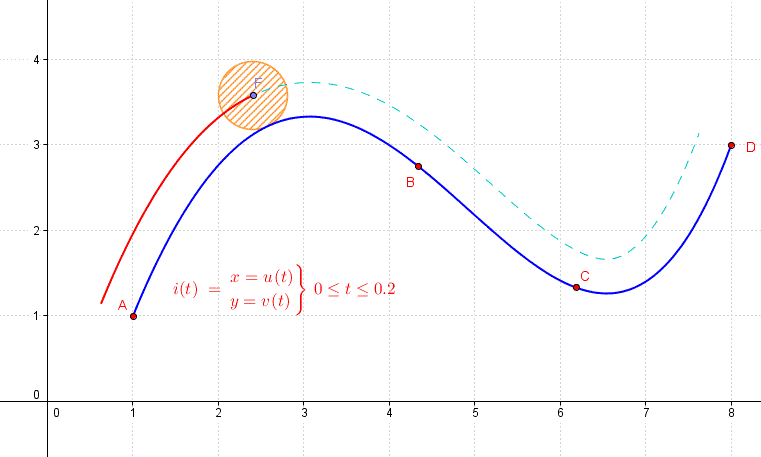
\includegraphics[scale=0.7]{imagens/FiguraTeste.png}
  	\vspace{-12pt}
  	\center {Fonte: Elaborada pelo autor}
  	\label{fig:FiguraTeste}
\end{figure}

De acordo com a figura 1, ...texto ...texto ...texto ...texto ...texto ...texto ...texto ...texto ...texto ...texto ...texto ...texto ...texto ...texto ...texto ...texto ...texto ...texto ...texto ...texto...texto ...texto ...texto ...texto

A Tabela 1 evidencia os dados...

\begin{table}[h]
	\centering
	\caption{Distância percorrida no intervalo 	de tempo entre 4 e 5 segundos}
	\begin{tabular}{c|c|c|c|c|c|c}
	\hline
	Intervalo de tempo (s) & 4,0 & 4,2 & 4,4  & 4,6 & 4,8 & 5,0 \\ \hline
	Distância (m) & 10,0 & 11,02 & 12,16  & 	13,45 & 14,96 & 16,80 \\  \hline  % não é preciso 	quebrar a última linha
	\end{tabular}
	\vspace{-10pt}
	\center {Fonte: Stewart (2012)}
\end{table}

A Equação \ref{eq1} mostra...%não dar enter
\begin{equation}\label{eq1}
P(t)={n \choose i}(1-t)^{n-i} t^i
\end{equation}


Detalhes adicionais sobre a como mencionar as figuras, as tabelas e as equações, o(a) candidato(a) deve consultar a norma NBR 14724.
